\documentclass[12pt]{article}
\usepackage{amsmath}
\usepackage{graphicx}
\usepackage{hyperref}
\usepackage{listings}
\usepackage{color}

\lstset{
    language=Python,                      % Set bahasa ke Python
    basicstyle=\ttfamily\footnotesize,    % Ukuran dan font kode
    keywordstyle=\color{blue},            % Warna keyword
    stringstyle=\color{red},              % Warna string
    commentstyle=\color{green},           % Warna komentar
    numbers=left,                         % Menampilkan nomor baris
    numberstyle=\tiny,                    % Ukuran nomor baris
    stepnumber=1,                         % Setiap baris diberi nomor
    breaklines=true,                      % Pemenggalan baris otomatis
    frame=single,                         % Bingkai di sekitar kode
    tabsize=4                             % Ukuran tab
}

\title{Operating System Course Report - First Half of the Semester}
\author{B class}
\date{\today}

\begin{document}

\maketitle
\newpage

\tableofcontents
\newpage

\section{Introduction}
This report summarizes the topics covered during the first half of the Operating System course. It includes theoretical concepts, practical implementations, and assignments. The course focuses on the fundamentals of operating systems, including system architecture, process management, CPU scheduling, and deadlock handling.

\section{Course Overview}
\subsection{Objectives}
The main objectives of this course are:
\begin{itemize}
    \item To understand the basic components and architecture of a computer system.
    \item To learn process management, scheduling, and inter-process communication.
    \item To explore file systems, input/output management, and virtualization.
    \item To study the prevention and handling of deadlocks in operating systems.
\end{itemize}

\subsection{Course Structure}
The course is divided into two halves. This report focuses on the first half, which covers:
\begin{itemize}
    \item Basic Concepts and Components of Computer Systems
    \item System Performance and Metrics
    \item System Architecture of Computer Systems
    \item Process Description and Control
    \item Scheduling Algorithms
    \item Process Creation and Termination
    \item Introduction to Threads
    \item File Systems
    \item Input and Output Management
    \item Deadlock Introduction and Prevention
    \item User Interface Management
    \item Virtualization in Operating Systems
\end{itemize}

\section{Topics Covered}

\subsection{Basic Concepts and Components of Computer Systems}
This section explains the fundamental components that make up a computer system, including the CPU, memory, storage, and input/output devices.

\subsection{System Performance and Metrics}
\subsubsection{\textit{Performance Metrics} Pada CPU}
\hspace*{1cm}Kalau kita membahas kinerja matriks pada komputer, maka kita tidak lepas dari CPU. CPU atau \textit{Central Processing Unit} adalah komponen utama dari komputer yang bertanggung jawab untuk mengeksekusi instruksi-instruksi yang diberikan kepada komputer. Kinerja sebuah sistem sangat dipengaruhi oleh bagaimana CPU mengeksekusi instruksi. Jika kita ingin memaksimalkan kinerja sebuah sistem, kita tentu perlu meminimalkan waktu eksekusi karena kinerja berbanding terbalik dengan waktu eksekusi.
\newline
\newline
\hspace*{1cm}Untuk menentukan waktu eksekusi CPU untuk sebuah program, Anda dapat mencari tahu jumlah total siklus clock yang dibutuhkan program dan mengalikannya dengan waktu siklus clock. Setiap program terdiri dari sejumlah instruksi dan setiap instruksi membutuhkan sejumlah siklus clock untuk dieksekusi. Jika Anda mengetahui jumlah total siklus clock per program dan mengetahui waktu siklus clock untuk setiap siklus clock ini, maka waktu eksekusi CPU dapat dihitung sebagai hasil perkalian jumlah total siklus clock CPU per program dengan waktu siklus clock. Karena waktu siklus clock dan clock rate saling terkait, hal ini juga dapat ditulis sebagai jumlah siklus clock CPU untuk sebuah program dibagi dengan clock rate.

\begin{figure}
    \centering
    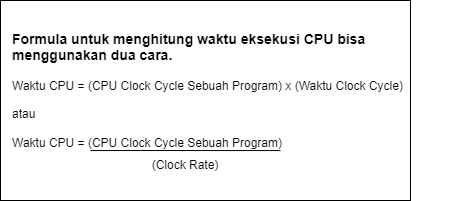
\includegraphics[width=\linewidth]{asset/image1.png}
    \caption{Rumus waktu CPU}
\end{figure}


\hspace*{1cm}Karena waktu eksekusi CPU merupakan hasil dari kedua faktor ini, kita dapat meningkatkan kinerja dengan mengurangi durasi waktu siklus clock atau jumlah siklus clock yang diperlukan untuk suatu program. Kecepatan clock pada dasarnya bergantung pada organisasi CPU tertentu.

\subsubsection{Mengapa \textit{Performance Metrics} Penting}
\hspace*{1cm}Mengukur kinerja menggunakan data yang akurat sangat penting dalam sebuah sistem karena memberikan gambaran nyata tentang performa yang sedang berlangsung. Dengan data yang tepat, manajemen dapat mengambil keputusan yang lebih terinformasi, sehingga memperkecil risiko kesalahan strategi. Selain itu, pengukuran kinerja juga membantu mengidentifikasi area yang membutuhkan perbaikan, sehingga organisasi dapat berfokus pada peningkatan yang signifikan. Memantau perkembangan dan kemajuan kinerja secara berkala meningkatkan akuntabilitas, baik di tingkat individu maupun tim, sehingga setiap anggota lebih bertanggung jawab atas hasil kerjanya. Pada akhirnya, penggunaan  \textit{performance metrics} yang tepat dapat mendorong peningkatan berkelanjutan, dengan memberikan dasar yang kuat bagi evaluasi dan inovasi secara sistematis dalam mencapai tujuan jangka panjang.

\subsection{System Architecture of Computer Systems}
Describes the architecture of modern computer systems, focusing on the interaction between hardware and the operating system.

\subsection{Process Description and Control}
Processes are a central concept in operating systems. This section covers:
\begin{itemize}
    \item Process states and state transitions
    \item Process control block (PCB)
    \item Context switching
\end{itemize}

\subsection{Scheduling Algorithms}
This section covers:
\begin{itemize}
    \item First-Come, First-Served (FCFS)
    \item Shortest Job Next (SJN)
    \item Round Robin (RR)
\end{itemize}
It explains how these algorithms are used to allocate CPU time to processes.

\subsection{Process Creation and Termination}
Details how processes are created and terminated by the operating system, including:
\begin{itemize}
    \item Process spawning
    \item Process termination conditions
\end{itemize}

\subsection{Introduction to Threads}
This section introduces the concept of threads and their relation to processes, covering:
\begin{itemize}
    \item Single-threaded vs. multi-threaded processes
    \item Benefits of multithreading
\end{itemize}

\subsection{File Systems}
File systems provide a way for the operating system to store, retrieve, and manage data. This section explains:
\begin{itemize}
    \item File system structure
    \item File access methods
    \item Directory management
\end{itemize}

\subsection{Input and Output Management}
Input and output management is key for handling the interaction between the system and external devices. This section includes:
\begin{itemize}
    \item Device drivers
    \item I/O scheduling
\end{itemize}

\subsection{Deadlock Introduction and Prevention}
Explores the concept of deadlocks and methods for preventing them:
\begin{itemize}
    \item Deadlock conditions
    \item Deadlock prevention techniques
\end{itemize}

\subsection{User Interface Management}
This section discusses the role of the operating system in managing the user interface. Topics covered include:
\begin{itemize}
    \item Graphical User Interface (GUI)
    \item Command-Line Interface (CLI)
    \item Interaction between the user and the operating system
\end{itemize}

\subsection{Virtualization in Operating Systems}
Virtualization allows multiple operating systems to run concurrently on a single physical machine. This section explores:
\begin{itemize}
    \item Concept of virtualization
    \item Hypervisors and their types
    \item Benefits of virtualization in modern computing
\end{itemize}

\section{Assignments and Practical Work}
\subsection{Assignment 1: Process Scheduling}
Students were tasked with implementing various process scheduling algorithms (e.g., FCFS, SJN, and RR) and comparing their performance under different conditions.

\subsection{Assignment 2: Deadlock Handling}
In this assignment, students were asked to simulate different deadlock scenarios and explore various prevention methods.

\subsection{Assignment 3: Multithreading and Amdahl's Law}
This assignment involved designing a multithreading scenario to solve a computationally intensive problem. Students then applied **Amdahl's Law** to calculate the theoretical speedup of the program as the number of threads increased.

\subsection{Assignment 4: Simple Command-Line Interface (CLI) for User Interface Management}
Students were tasked with creating a simple **CLI** for user interface management. The CLI should support basic commands such as file manipulation (creating, listing, and deleting files), process management, and system status reporting.

\subsection{Assignment 5: File System Access}
In this assignment, students implemented file system access routines, including:
\begin{itemize}
    \item File creation and deletion
    \item Reading from and writing to files
    \item Navigating directories and managing file permissions
\end{itemize}

\section{Conclusion}
The first half of the course introduced core operating system concepts, including process management, scheduling, multithreading, and file system access. These topics provided a foundation for more advanced topics to be covered in the second half of the course.

\begin{thebibliography}{9}
    \bibitem{gfg2024}
    GeeksforGeeks. (n.d.). Computer organization: Performance of computer. GeeksforGeeks. Retrieved October 1, 2024, from https://www.geeksforgeeks.org/computer-organization-performance-of-computer/
    \end{thebibliography}

\end{document}